% Options for packages loaded elsewhere
\PassOptionsToPackage{unicode}{hyperref}
\PassOptionsToPackage{hyphens}{url}
%
\documentclass[
]{article}
\usepackage{amsmath,amssymb}
\usepackage{lmodern}
\usepackage{iftex}
\ifPDFTeX
  \usepackage[T1]{fontenc}
  \usepackage[utf8]{inputenc}
  \usepackage{textcomp} % provide euro and other symbols
\else % if luatex or xetex
  \usepackage{unicode-math}
  \defaultfontfeatures{Scale=MatchLowercase}
  \defaultfontfeatures[\rmfamily]{Ligatures=TeX,Scale=1}
\fi
% Use upquote if available, for straight quotes in verbatim environments
\IfFileExists{upquote.sty}{\usepackage{upquote}}{}
\IfFileExists{microtype.sty}{% use microtype if available
  \usepackage[]{microtype}
  \UseMicrotypeSet[protrusion]{basicmath} % disable protrusion for tt fonts
}{}
\makeatletter
\@ifundefined{KOMAClassName}{% if non-KOMA class
  \IfFileExists{parskip.sty}{%
    \usepackage{parskip}
  }{% else
    \setlength{\parindent}{0pt}
    \setlength{\parskip}{6pt plus 2pt minus 1pt}}
}{% if KOMA class
  \KOMAoptions{parskip=half}}
\makeatother
\usepackage{xcolor}
\IfFileExists{xurl.sty}{\usepackage{xurl}}{} % add URL line breaks if available
\IfFileExists{bookmark.sty}{\usepackage{bookmark}}{\usepackage{hyperref}}
\hypersetup{
  pdftitle={Relaxation Layer},
  hidelinks,
  pdfcreator={LaTeX via pandoc}}
\urlstyle{same} % disable monospaced font for URLs
\usepackage{longtable,booktabs,array}
\usepackage{calc} % for calculating minipage widths
% Correct order of tables after \paragraph or \subparagraph
\usepackage{etoolbox}
\makeatletter
\patchcmd\longtable{\par}{\if@noskipsec\mbox{}\fi\par}{}{}
\makeatother
% Allow footnotes in longtable head/foot
\IfFileExists{footnotehyper.sty}{\usepackage{footnotehyper}}{\usepackage{footnote}}
\makesavenoteenv{longtable}
\usepackage{graphicx}
\makeatletter
\def\maxwidth{\ifdim\Gin@nat@width>\linewidth\linewidth\else\Gin@nat@width\fi}
\def\maxheight{\ifdim\Gin@nat@height>\textheight\textheight\else\Gin@nat@height\fi}
\makeatother
% Scale images if necessary, so that they will not overflow the page
% margins by default, and it is still possible to overwrite the defaults
% using explicit options in \includegraphics[width, height, ...]{}
\setkeys{Gin}{width=\maxwidth,height=\maxheight,keepaspectratio}
% Set default figure placement to htbp
\makeatletter
\def\fps@figure{htbp}
\makeatother
\setlength{\emergencystretch}{3em} % prevent overfull lines
\providecommand{\tightlist}{%
  \setlength{\itemsep}{0pt}\setlength{\parskip}{0pt}}
\setcounter{secnumdepth}{-\maxdimen} % remove section numbering
\ifLuaTeX
  \usepackage{selnolig}  % disable illegal ligatures
\fi

\title{Relaxation Layer}
\author{}
\date{}

\begin{document}
\maketitle

\hypertarget{evaluation-of-the-relaxation-layer-past-a-normal-shockwave-using-monti-napolitano-model}{%
\section{Evaluation of the Relaxation layer past a Normal shockWave
using Monti-Napolitano
model}\label{evaluation-of-the-relaxation-layer-past-a-normal-shockwave-using-monti-napolitano-model}}

Downstream a Normal shock wave, whom upstream mach number is in the
hypersonic regime, the flow can reach hign enough temperatures that
don't allow us to consider the gas in thermodynamic equilibrium.\\
We have to consider the finite rate chemical processes that modify the
thermofluidynamics properties oof the gas.\\
In particular we can address the importance of this chemical processes
on the flow by evaluating the Damkoeler number: \[
Da=\frac{\text{transport time species}}{\text{chemical reaction time}}=\frac{t_m}{t_r}
\] and we can define 3 limiting cases: - \(Da<<1\), frozen gas -
\(Da\simeq 1\), non equilibbrium - \(Da>>1\), istantaneous equilibrium

When considering the flow trough a shock wave, since it's only a few
mean free path thick, the gas can be considered to be in a frozen state,
thus the Rankine-Hugonoit equations do apply.\\
At this boundary of the relaxation layer the thermo-fluidynamic
properties of the gas are the ones prescribed by the Rankine-hugonoit
equations for the frozen state of the gas. Then it evolves towards
equilibrium.\\
When the gas is air in principle whe should consider: - exitation of
vibrational state of \(N_2\) - dissociation of \(O_2\), \(N_2\), and
subsequent formation o atomic oxigen, nitrogen and \(NO\) - ionization

\hypertarget{monti-napolitano-model}{%
\subsection{Monti-Napolitano model}\label{monti-napolitano-model}}

In the present discussion the model is simplyfied by the assumption that
\(N_2\) does not dissociate and no ionization is involved. This lead to
the Monti-Napolitano model. It is thus valid for a range of temperature
well above the vibrational temperature of \(O_2\), \(T_v=2279K\) and
well below the dissotiation temperature of \(N_2\), \(T_d=113159K\).\\
For the problem of the relaxation layer past a normal shock wave, this
model is accurate enough for shock such that: \[
\frac {T_2}{T_1}<15 \quad \frac{\rho_2}{\rho_1}<10
\] and thus limits its applicability for a specific set of range of
altitudes and Mach number. This model assume that:

\begin{itemize}
\tightlist
\item
  the vibrational,rotational and traslational degrees of freedom of
  \(O2\), the traslational, rotational degrees of freedom of \(N2\), the
  traslational d.o.f of \(O\) are in equlibrium at temperature T
\item
  the vibrational degrees of freedom of \(N_2\) are in equilibrium at
  temperature \(T_v\)
\item
  for the vibrational d.o.f of \(O_2\) is used the partition function of
  the Lighthill oscillator
\item
  the dissotiation of \(O_2\) is carachterized via the the mass fraction
  \(\alpha\), and \(T_\alpha\) is rapresentative of the dissociation
  energy of the molecular oxigen
\end{itemize}

So it can be considered a model defined by 3 temperature. The equation
to describe the evolution of the \(T_v\) and \(\alpha\) are described in
the following section.

\hypertarget{chemical-rate-equation}{%
\subsubsection{Chemical rate equation}\label{chemical-rate-equation}}

We must consider the following reactions, at varing \(M\), \[
O_2 + M  \leftrightarrow 2O + M
\]

thus we have 3 reactions, for \(M\) equal to \(O\), \(O_2\) or \$
N\_2\$. the chemical rate equation, expressed via molar concentration
is: \[
\frac{d[O]}{dt}=K_d[O_2][M] - K_r[O]^2[M]
\] that can be expressed using the equilibrum constant
\(K=\frac{K_d}{K_r}\). \[
\frac{d[O]}{dt}=K_r(K[O_2][M] - [O]^2[M])
\] More work is needed to express it using the masss fraction \(\alpha\)

\hypertarget{vibrational-temperature-equation}{%
\subsubsection{vibrational Temperature
equation}\label{vibrational-temperature-equation}}

The evolution of the vibrational Temperature of \(N_2\) is described by
the following equation of in the Entropy of the vibrational dof of
\(N_2\): \[
T_v\frac{dS_v}{dt}=\frac{1}{t_c} [E_v(T) - E_v(T_v)]
\] which togheter with the equation of the entropy \[
S=k(1 +\ln\frac Q N )+ \frac{E-E_0}{T}
\]

lead to an ODE for \(T_v\).

\hypertarget{model-and-computation}{%
\subsection{model and computation}\label{model-and-computation}}

To solve the relaxation layer past a normal shock wave we know that: -
the mass is conserved - the impulse is conserved - The flow is
homoentalpic - the gas is in non equilibrium - we assume valid the
Monti-Napolitano Model

thus we can consider the set of equations formed by the following: -
total mass conservation - momentum balance - energy conservation -
equation of state of the gas for the pressure - equation of state of the
internal energy - vibrational Temperature equation - Chemical rate
equation

these form a closed set of equation that can be integrated, for example
with a runge-kutta method until equilibrium is reached.

\hypertarget{results}{%
\subsection{Results}\label{results}}

The relaxation layer was computed for two altitude and mach number.

\begin{longtable}[]{@{}llllllll@{}}
\toprule
Ma & gamma & R {[}J/Kg K{]} & T {[}K{]} & rho {[}Kg/m\^{}3{]} & p
{[}Pa{]} & n & h {[}km{]} \\
\midrule
\endhead
6.4 & 1.4 & 287.05 & 250 & 0.004 & 290 & 5 & 40 \\
8.3 & 1.4 & 287.05 & 264 & 0.002 & 150 & 5 & 45 \\
\bottomrule
\end{longtable}

\hypertarget{km-altitude-case}{%
\subsubsection{40 Km altitude case}\label{km-altitude-case}}

In this case we can observe how \(T_v\), \(T\), \(\alpha\) and
equlibrium concentration of atomic oxigen \(\alpha_e\) evolve in the
relaxation layer. The location at wich first \(T_v\) reaches \(T\) the
vibrational d.o.f of nitrogen comes at equilibrium with the other d.o.f
of the gas, we can call this condition partial equilibrium. Much further
also equilibrium in the concentration of atomic oxigen is
accomplished.\\
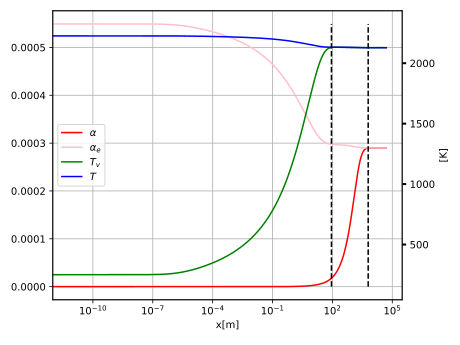
\includegraphics{images/40km/NequilibriumFlowNSW_T_alpha.svg}

the following profiles of the thermo-fluidynamic quantities are obtained

\includegraphics{images/40km/NequilibriumFlowNSW_u.svg}\\
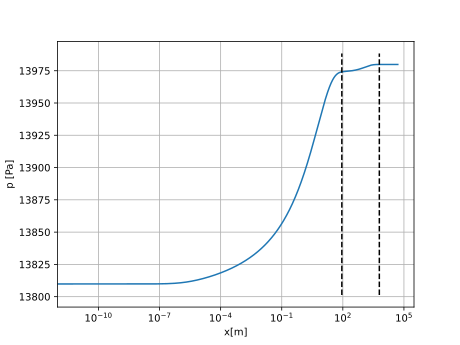
\includegraphics{images/40km/NequilibriumFlowNSW_p.svg}\\
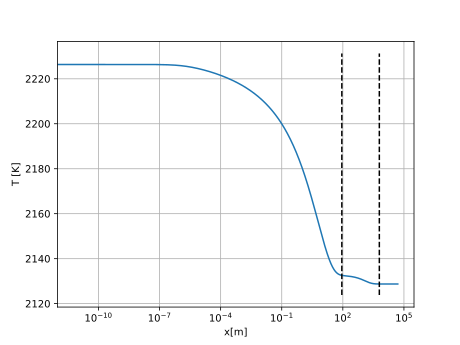
\includegraphics{images/40km/NequilibriumFlowNSW_T.svg}\\
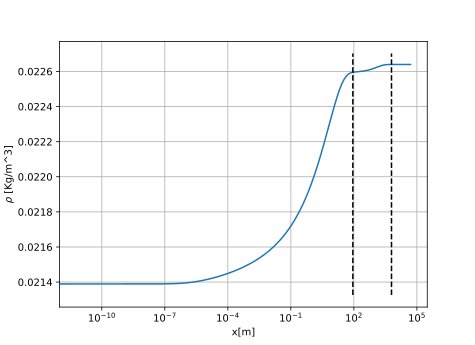
\includegraphics{images/40km/NequilibriumFlowNSW_rho.svg}

We can observe that the evolution of the vibrational d.o.f of \(N_2\)
influence much more than \(\alpha\) the evolution of the thermodynamic
quantities. The Temperature \(T\) decreases since the excitement of the
vibrational state is an endothermic reaction. Most of the overall
kinetic energy content of the gas is lost in the vibrational excitement,
we can see how the velocity \(u\) drops as partial equilibrium is
reached, and thus increasing the sensible hentalpy of the mixture.\\
Then density and pressure increase because of the conservation of mass
and impulse.

\hypertarget{km-altitude-case-1}{%
\subsubsection{45 Km altitude case}\label{km-altitude-case-1}}

The behaviour of the thermo-fluid dynamic quantities are similar to the
case at 40 Km. This time partial and complete equilibrium are
accomplished almost at the same location.

\begin{figure}
\centering
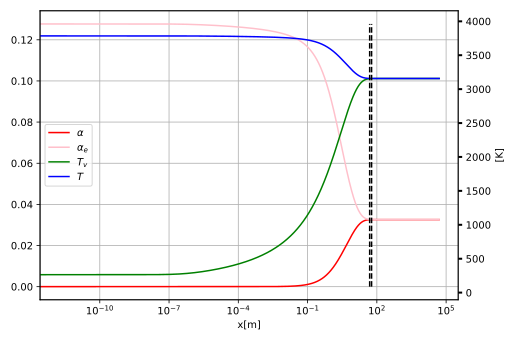
\includegraphics{images/45km/NequilibriumFlowNSW_T_alpha.svg}
\caption{``equilibium at 45km''}
\end{figure}

the following profiles of the thermo-fluidynamic quantities are obtained

\includegraphics{images/45km/u.svg}\\
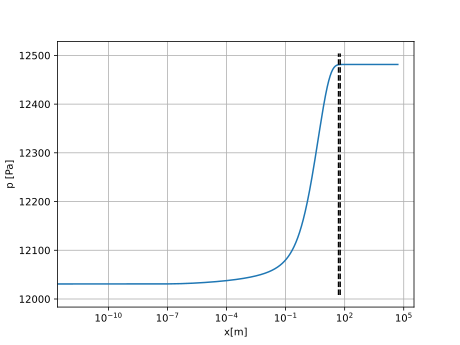
\includegraphics{images/45km/p.svg}\\
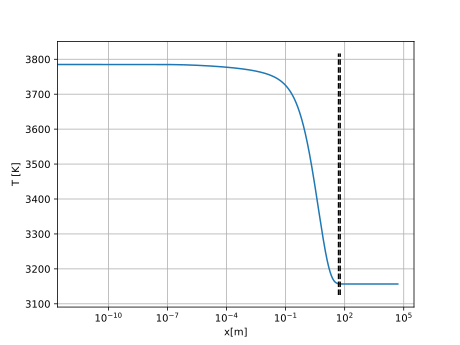
\includegraphics{images/45km/T.svg}\\
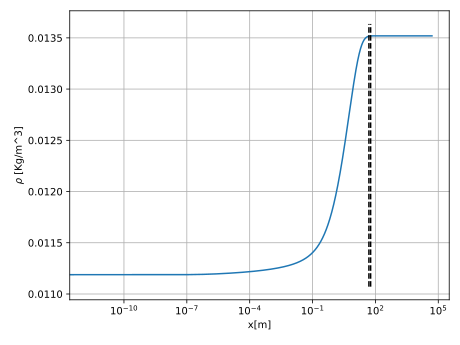
\includegraphics{images/45km/rho.svg}

\hypertarget{note}{%
\subsubsection{Note}\label{note}}

\begin{quote}
the fact that vibrational d.o.f equilibrium is systematically reached
before the equilibrium in dissotiation mass fraction \(\alpha\) is
beacause thermal equilibrium is fondamentally due to collision between
particles and the excitment of the vibrational d.o.f require far less
energy, and thus collisions, in contrast to the dissociation reactions
\end{quote}

\end{document}
